\clearpage
\begin{flushright}
	\textit{Лекция №24}
	\textit{2015.12.22}
\end{flushright}

Реализация обработки прерываний в системе:
\begin{enumerate}
    \item запрещение прерывание (для многопроцессорных систем запрещение прерываний выполняется на локальном процессоре; в системе столько таблиц дескрипторов прерываний (таблиц диспетчеризации прерываний) сколько процессоров, так как каждый процессор должен адресовать возникающее прерывание; только прерывание от системного таймера выполняется одним процессором и такой процессор принято называть главным, несмотря на симметричность системы). 
    \item вложенные прерывания (предполагают наличие приоритетов и в соответствии с этими приоритетами более высокоприоритетные прерывания вытесняют менее приоритетные; контекст сохраняется либо в стековой ??? либо в стеке). 
\end{enumerate} 

Файловые системы. Современные системы отличаются только файловыми системами. Имеют уровни иерархии. Самый верхний – символьный уровень именования файлов. Доступ к дискам осуществляется через подсистему ввода/вывода.  ФС позволяет единообразно работать с устройствами. 


\chapter{ОС реального времени}

Определение Posix: 
Реальное время в операционных системах – способность ОС обеспечить требуемый уровень сервиса в определенный промежуток времени. 
Перефразируем: ОС должна обеспечить возможность обслуживать внешние по отношению к системе системы за определенный промежуток времени. У нас есть некое устройство/система устройств и мы должны обеспечить управление ими. 
В системах общего назначения windows/Linux обеспечивают управление процессами реального времени, однако ключевым отличием сервисов ядра ОС реального времени является детерминированный характер их работы, основанный на строгом контроле времени выполнения определенных задач. Под детерминированностью следует понимать хорошо изученные системы, т.е. все системы реального времени являются системами специального назначения. Даже QNX, когда настроена на выполнение конкретным объектом (имеет все возможности) становится системой специального назначения. Про этот объект следует знать все о процессах и потоках. 

Различаются два типа реального времени:
\begin{enumerate}
    \item жесткое (предполагает ответ системы в строго отведенный интервал времени);
    \item мягкое (возможны задержки).
\end{enumerate} 

Системы реального времени строятся по определенным принципам:
\begin{enumerate}
    \item алгоритмы, позволяющие обеспечивать быстрое переключение потоков (переключение контекста должно выполняться быстро, должно поддерживаться аппаратно) 
    \item минимальные временные задержки
\end{enumerate} 

Способы построения систем РВ:
\begin{enumerate}
    \item на основе событийной синхронизации, которая предполагает переключение задач только тогда, когда возникает событие с более высоким приоритетом. Такой приоритет называется приоритетом планирования.
    \item квантование.
\end{enumerate} 

В системах реального времени главным критерием эффективности является обеспечение временных характеристик вычислительно процесса. В этих системах планирование имеет особое значение. Любая система РВ должна реагировать на сигналы управляемого объекта в течение заданных временных интервалов. Необходимость тщательного планирования работ облегчается тем, что весь набор выполняемых задач известен заранее. Чтобы система могла эффективно управлять набором задач в системе должна иметься информация не только о времени выполнения, но и о текущих затратах времени, о моментах активации задач и о предельно допустимых интервалов ожидания ответа. В системах реального времени применяются как статические приоритеты и алгоритмы планирования на статических приоритетах, так и динамические приоритеты и соответствующие алгоритмы. Появились недавно, связано это с ростом мощности компов. 

Система резервирования билетов – мягкая система. Если из-за временных нарушений оператору не удается зарезервировать билет, то можно повторить заново. 

QNX NEUTRINO v6.2 - ОС с микроядерной архитектурой построенная на модели клиент-сервер. Процесс в этой системе взаимодействуют с помощью сообщений. Поддерживает виртуальную память. Управление виртуальной памятью является затратным.

QNX обеспечивают все составляющие систем РВ:
\begin{enumerate}
    \item многозадачность;
    \item диспетчеризацию потоков на основе приоритетов;
    \item быстрое переключение контекста;
    \item вложенные прерывания
\end{enumerate} 

\begin{figure}[H]
    \centering
    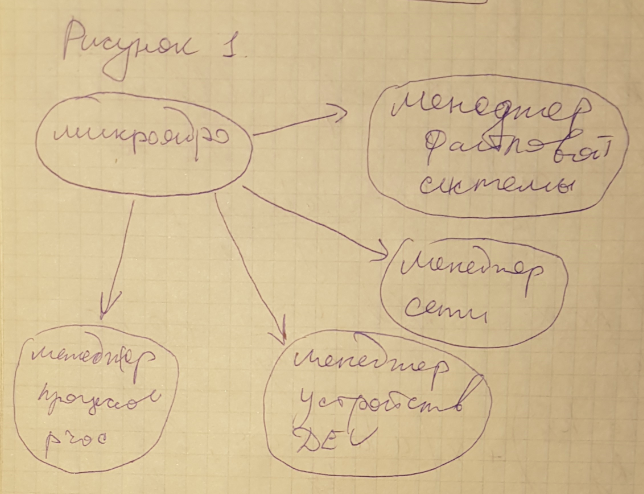
\includegraphics[width=\textwidth]{pic/1.png}
    \caption{Структура}
\end{figure}

Особенность микроядра - в отдельные модули вынесена поддержка управления дисками, управления  сетевыми возможностями, при этом запуск и работа модулей аналогична пользовательским процессам. 

Ядро выполняет функции:
\begin{enumerate}
    \item передачу сообщений (обеспечивает маршрутизацию сообщений);
    \item диспетчеризация потоков (простейший процесс имеет один поток).
\end{enumerate} 

Переключение потоков и процессов мало чем отличается. 
Процесс в QNX выполняется в собственном виртуальном адресном пространстве. Само ядро никогда не получает управление в результате диспетчеризации. Код ядра выполняется только как следствие системных вызовов, исключений или аппаратных прерываний. Единица диспетчеризации – поток.

Существует три события, в результате которых выполняется диспетчеризация потоков:
\begin{enumerate}
    \item вытеснение; 
    \item блокирование (выполняемый поток может вызвать функцию, которая приведет к его блокировке);
    \item уступка. 
\end{enumerate} 

Поток в системе может иметь два состояния:
\begin{enumerate}
    \item готов;
    \item заблокирован.
\end{enumerate} 

Планирование потоков выполняется на основе системы приоритетов. Для супер-юзера выделен специальный диапазон приоритетов. Весь: 0-255. Пользовательский: 0 – 63.

Поддерживает дисциплины планирования:
\begin{enumerate}
    \item FIFO (поток выполняется пока не будет вытеснен более приоритетным/заблокируется/добровольно отдаст);
    \item RR (поток выполняется в течении определенного кванта; квант в 4 раза больше тактового интервала; тактовый интервал 1мс в процессорах с тактовой частотой 40МГц; в х86 квант будет 4мс);
    \item спорадическая (случайное) (вводится понятие приоритет переднего плана foreground и фоновый background) 
\end{enumerate} 

Для управления спорадическим подходом используется:
\begin{enumerate}
    \item кол-во времени, за которое поток может выполниться;
    \item до какого уровня можно понизить приоритет
    \item период пополнения, когда поток может расходовать свой бюджет выполнения;
    \item максимально число текущих пополнений.
\end{enumerate} 

\begin{figure}[H]
    \centering
    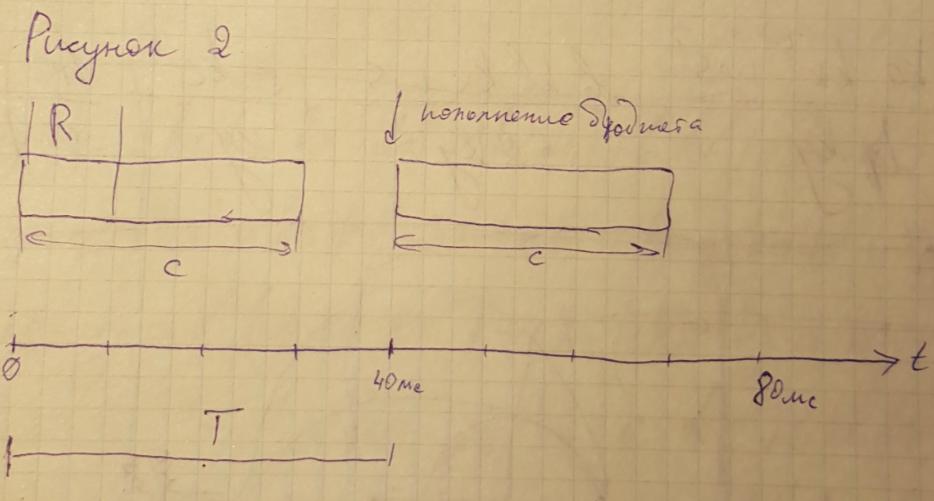
\includegraphics[width=\textwidth]{pic/2.png}
    \caption{pic}
\end{figure}

$C$ – начальный бюджет выполнения потока, который расходуется потоком в процессе выполнения. Бюджет пополняется с периодичностью $Т$. Когда поток блокируется, израсходованная часть потока $R$ пополняется. 
Если в каком-то из драйверов возникла ошибка, то это не приводит к перезапуску системы, а приводит к перезапуску драйвера. 

\chapter{Точные и неточные прерывания}
Cвязано с суперскалярными процессорами.

\begin{figure}[H]
    \centering
    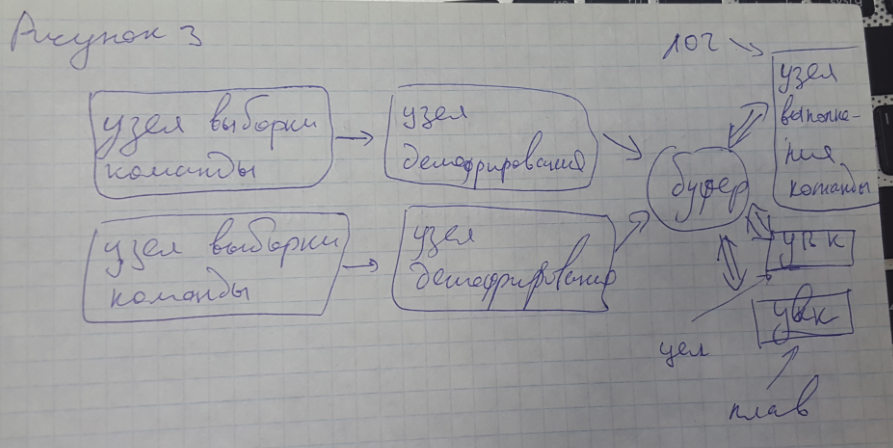
\includegraphics[width=\textwidth]{pic/3.png}
    \caption{Диаграмма выполнения команды}
\end{figure}

Команды могут выполняться не последовательно. В структуре с конвейером различные команды находятся на разных стадиях выполнения. В момент прерывания значение счетчика команд может не отражать истинной границы между выполненными и еще не выполненными командами. Скорее всего, он будет указывать на следующую команду, какую нужно считать из памяти. Соответственно при возврате и прерывания ОС не может просто начать заполнять конвейер с команды указанной в адресе счетчика команд.  Она должна определить последнюю выполненную команду, что требует проведения серьезного анализа процессора. В суперскалярной еще хуже, поскольку команды могут выполняться не в порядке их расположения в памяти, нет четкой границы между невыполненными и выполненными. 
Может возникнуть такая ситуация: команды 1,2,3,5,8 – выполнены, 4,6,7,9,10 – не выполнены. Счетчик команд может указывать на 9, 10 или 11 команды. Вводится понятие \textbf{точного прерывания} – это прерывание, которое оставляет машину в строго определенном состоянии. 

Свойства точного прерывания:
\begin{enumerate}
    \item счетчик команд указывает на команду, до которой все команды полностью выполнены;
    \item ни одна команда, после той, на которую указывает счетчик команд – не выполнены;
    \item состояние команды, на которую указывает счетчик команд – известно. 
\end{enumerate} 
    
Ничего не говорится о том, что команды после той, на которую указывает счетчик команд, не могли начаться, утверждается только, что все изменения, связанные с выполнением этих команд, должны быть отменены до начала обработки прерывания.
